%!TEX program = xelatex
\documentclass{beamer}

%
% Common preamble for all three parts.
%
\usepackage{ifxetex}
\ifxetex
  \usepackage{polyglossia}
    \setdefaultlanguage{brazil}
    \usefonttheme{professionalfonts}
  \usepackage{fontspec}
  \usepackage{unicode-math}
\else
  \usepackage[brazil]{babel}
  \usepackage[T1]{fontenc}
  \usepackage[utf8]{inputenc}
\fi

\usepackage{amsmath}
\usepackage{color}
\usepackage{minted}
\usepackage{hyperref}
\usepackage{multicol}
\usepackage{graphicx}
\usepackage{tabularx}
\usepackage{tikz}

% only inline todonotes work
\usepackage{xkeyval}
\usepackage[textsize=small]{todonotes}
\presetkeys{todonotes}{inline}{}

\usetikzlibrary{shapes,arrows,positioning,shadows}

% no nav buttons
\usenavigationsymbolstemplate{}

\newcommand{\bftt}[1]{\textbf{\texttt{#1}}}
\newcommand{\comment}[1]{{\color[HTML]{008080}\textit{\textbf{\texttt{#1}}}}}
\newcommand{\cmd}[1]{{\color[HTML]{008000}\bftt{#1}}}
\newcommand{\bs}{\char`\\}
\newcommand{\cmdbs}[1]{\cmd{\bs#1}}
\newcommand{\lcb}{\char '173}
\newcommand{\rcb}{\char '175}
\newcommand{\cmdbegin}[1]{\cmdbs{begin\lcb}\bftt{#1}\cmd{\rcb}}
\newcommand{\cmdend}[1]{\cmdbs{end\lcb}\bftt{#1}\cmd{\rcb}}

\newcommand{\wllogo}{\textbf{Overleaf}}

% this is where the example source files are loaded from
% do not include a trailing slash
\newcommand{\fileuri}{https://raw.github.com/guibeal/latex-course/master/pt-br}

\newcommand{\wlserver}{https://www.overleaf.com}
\newcommand{\wlnewdoc}[1]{\wlserver/docs?snip\_uri=\fileuri/#1\&splash=none}

\def\tikzname{Ti\emph{k}Z}

% from http://tex.stackexchange.com/questions/5226/keyboard-font-for-latex
\newcommand*\keystroke[1]{%
  \tikz[baseline=(key.base)]
    \node[%
      draw,
      fill=white,
      drop shadow={shadow xshift=0.25ex,shadow yshift=-0.25ex,fill=black,opacity=0.75},
      rectangle,
      rounded corners=2pt,
      inner sep=1pt,
      line width=0.5pt,
      font=\scriptsize\sffamily
    ](key) {#1\strut}
  ;
}
\newcommand{\keystrokebftt}[1]{\keystroke{\bftt{#1}}}

% stolen from minted.dtx
\newenvironment{exampletwoup}
  {\VerbatimEnvironment
   \begin{VerbatimOut}{example.out}}
  {\end{VerbatimOut}
   \setlength{\parindent}{0pt}
   \fbox{\begin{tabular}{l|l}
   \begin{minipage}{0.55\linewidth}
     \inputminted[fontsize=\small,resetmargins]{latex}{example.out}
   \end{minipage} &
   \begin{minipage}{0.35\linewidth}
     \input{example.out}
   \end{minipage}
   \end{tabular}}}

\newenvironment{exampletwouptiny}
  {\VerbatimEnvironment
   \begin{VerbatimOut}{example.out}}
  {\end{VerbatimOut}
   \setlength{\parindent}{0pt}
   \fbox{\begin{tabular}{l|l}
   \begin{minipage}{0.55\linewidth}
     \inputminted[fontsize=\scriptsize,resetmargins]{latex}{example.out}
   \end{minipage} &
   \begin{minipage}{0.35\linewidth}
     \setlength{\parskip}{6pt plus 1pt minus 1pt}%
     \raggedright\scriptsize\input{example.out}
   \end{minipage}
   \end{tabular}}}

\newenvironment{exampletwouptinynoframe}
  {\VerbatimEnvironment
   \begin{VerbatimOut}{example.out}}
  {\end{VerbatimOut}
   \setlength{\parindent}{0pt}
   \begin{tabular}{l|l}
   \begin{minipage}{0.55\linewidth}
     \inputminted[fontsize=\scriptsize,resetmargins]{latex}{example.out}
   \end{minipage} &
   \begin{minipage}{0.35\linewidth}
     \setlength{\parskip}{6pt plus 1pt minus 1pt}%
     \raggedright\scriptsize\input{example.out}
   \end{minipage}
   \end{tabular}}

\title{Uma Introdução Interativa ao \LaTeX}
\author{
  Dr John D. Lees-Miller
  \texorpdfstring{\\[2mm]}{}
  Tradução: Dr Luiz-Rafael Santos
  \texorpdfstring{\\[2mm]}{}
  Adaptação: Guilherme de P. Beal
}
\titlegraphic{%
  \includegraphics[height=30pt]{overleaf}
  \\[0.75mm]
  
\includegraphics[height=45pt]{ufrgs}
  \qquad
  
\includegraphics[height=45pt]{ceeca}
}

\makeatletter
\define@key{PAX@Gin}{scale}{}
\makeatother


\subtitle{Parte 2: Documentos Estruturados \& Muito Mais}

\begin{document}

%%%%%%%%%%%%%%%%%%%%%%%%%%%%%%%%%%%%%%%%%%%%%%%%%%%%%%%%%%%%%%%%%%%%%%%%%%%%%%%
%%%%%%%%%%%%%%%%%%%%%%%%%%%%%%%%%%%%%%%%%%%%%%%%%%%%%%%%%%%%%%%%%%%%%%%%%%%%%%%
%%%%%%%%%%%%%%%%%%%%%%%%%%%%%%%%%%%%%%%%%%%%%%%%%%%%%%%%%%%%%%%%%%%%%%%%%%%%%%%
\begin{frame}
\titlepage
\end{frame}

%%%%%%%%%%%%%%%%%%%%%%%%%%%%%%%%%%%%%%%%%%%%%%%%%%%%%%%%%%%%%%%%%%%%%%%%%%%%%%%
%%%%%%%%%%%%%%%%%%%%%%%%%%%%%%%%%%%%%%%%%%%%%%%%%%%%%%%%%%%%%%%%%%%%%%%%%%%%%%%
%%%%%%%%%%%%%%%%%%%%%%%%%%%%%%%%%%%%%%%%%%%%%%%%%%%%%%%%%%%%%%%%%%%%%%%%%%%%%%%
\section{Documentos Estruturados}

%%%%%%%%%%%%%%%%%%%%%%%%%%%%%%%%%%%%%%%%%%%%%%%%%%%%%%%%%%%%%%%%%%%%%%%%%%%%%%%
%%%%%%%%%%%%%%%%%%%%%%%%%%%%%%%%%%%%%%%%%%%%%%%%%%%%%%%%%%%%%%%%%%%%%%%%%%%%%%%
%%%%%%%%%%%%%%%%%%%%%%%%%%%%%%%%%%%%%%%%%%%%%%%%%%%%%%%%%%%%%%%%%%%%%%%%%%%%%%%
\begin{frame}{Sumário}
\begin{multicols}{2}
\tableofcontents[currentsection]
\end{multicols}
\end{frame}

%%%%%%%%%%%%%%%%%%%%%%%%%%%%%%%%%%%%%%%%%%%%%%%%%%%%%%%%%%%%%%%%%%%%%%%%%%%%%%%
%%%%%%%%%%%%%%%%%%%%%%%%%%%%%%%%%%%%%%%%%%%%%%%%%%%%%%%%%%%%%%%%%%%%%%%%%%%%%%%
%%%%%%%%%%%%%%%%%%%%%%%%%%%%%%%%%%%%%%%%%%%%%%%%%%%%%%%%%%%%%%%%%%%%%%%%%%%%%%%
\begin{frame}{\insertsection}
\begin{itemize}
  \item Na Parte 1, aprendemos como utilizar comandos e ambientes para digitar textos, matemáticos ou não.
  \item Agora, aprenderemos a utilizar comandos e ambientes para estruturar documentos.
  \item Você deve tentar os novos comandos no Overleaf:
\end{itemize}
\vskip 2em
\begin{center}
\fbox{\href{\wlnewdoc{basics.tex}}{Clique aqui para abrir o documento-exemplo no \wllogo{}}}
\\[1ex]\scriptsize{}
\end{center}
\vskip 2ex
\begin{itemize}
  \item Vamos começar!
\end{itemize}
\end{frame}

%%%%%%%%%%%%%%%%%%%%%%%%%%%%%%%%%%%%%%%%%%%%%%%%%%%%%%%%%%%%%%%%%%%%%%%%%%%%%%%
%%%%%%%%%%%%%%%%%%%%%%%%%%%%%%%%%%%%%%%%%%%%%%%%%%%%%%%%%%%%%%%%%%%%%%%%%%%%%%%
%%%%%%%%%%%%%%%%%%%%%%%%%%%%%%%%%%%%%%%%%%%%%%%%%%%%%%%%%%%%%%%%%%%%%%%%%%%%%%%
\subsection{Título e Resumo}
\begin{frame}[fragile]{\insertsubsection}
\begin{itemize}{\small
  \item Informe ao \LaTeX{} no preâmbulo o título, usando o comando \cmdbs{title} e o autor, usando o comando \cmdbs{author}.
  \item Então use \cmdbs{maketitle} no documento para realmente criar o título.
  \item Use o ambiente \bftt{abstract} para criar um resumo.
}\end{itemize}
\begin{minipage}{0.45\linewidth}
  \inputminted[fontsize=\tiny,frame=single,resetmargins]{latex}{structure-title.tex}
\end{minipage}
\begin{minipage}{0.45\linewidth}
  \includegraphics[width=\textwidth,clip,trim=2.2in 7in 2.2in 2in]{structure-title.pdf}
\end{minipage}
\end{frame}

%%%%%%%%%%%%%%%%%%%%%%%%%%%%%%%%%%%%%%%%%%%%%%%%%%%%%%%%%%%%%%%%%%%%%%%%%%%%%%%
%%%%%%%%%%%%%%%%%%%%%%%%%%%%%%%%%%%%%%%%%%%%%%%%%%%%%%%%%%%%%%%%%%%%%%%%%%%%%%%
%%%%%%%%%%%%%%%%%%%%%%%%%%%%%%%%%%%%%%%%%%%%%%%%%%%%%%%%%%%%%%%%%%%%%%%%%%%%%%%
\subsection{Seções}
\begin{frame}{\insertsubsection}
\begin{itemize}{\small
  \item Utilize os comandos \cmdbs{section} e \cmdbs{subsection} para criar seções e subseções.
  \item Você pode adivinhar o que os comandos \cmdbs{section*} e \cmdbs{subsection*} fazem?
}\end{itemize}
\begin{minipage}{0.45\linewidth}
  \inputminted[fontsize=\tiny,frame=single,resetmargins]{latex}{structure-sections.tex}
\end{minipage}
\begin{minipage}{0.45\linewidth}
  \expandafter\includegraphics\expandafter[width=\textwidth,clip,trim=1.5in 6in 3.5in 1in]{structure-sections.pdf}
\end{minipage}
\end{frame}

%%%%%%%%%%%%%%%%%%%%%%%%%%%%%%%%%%%%%%%%%%%%%%%%%%%%%%%%%%%%%%%%%%%%%%%%%%%%%%%
%%%%%%%%%%%%%%%%%%%%%%%%%%%%%%%%%%%%%%%%%%%%%%%%%%%%%%%%%%%%%%%%%%%%%%%%%%%%%%%
%%%%%%%%%%%%%%%%%%%%%%%%%%%%%%%%%%%%%%%%%%%%%%%%%%%%%%%%%%%%%%%%%%%%%%%%%%%%%%%
\subsection{Rótulos e Referência Cruzada}
\begin{frame}[fragile]{\insertsubsection}
\begin{itemize}{\small
  \item Use \cmdbs{label} para rotular e \cmdbs{ref} para referência cruzada automática.
  \item O pacote \bftt{amsmath} disponibiliza o comando \cmdbs{eqref} para referenciar equações.
}\end{itemize}
\begin{minipage}{0.45\linewidth}
  \inputminted[fontsize=\tiny,frame=single,resetmargins]{latex}{structure-crossref.tex}
\end{minipage}
\begin{minipage}{0.45\linewidth}
  \includegraphics[width=\textwidth,clip,trim=1.8in 6in 1.625in 1in]{structure-crossref.pdf}
\end{minipage}
\end{frame}

%%%%%%%%%%%%%%%%%%%%%%%%%%%%%%%%%%%%%%%%%%%%%%%%%%%%%%%%%%%%%%%%%%%%%%%%%%%%%%%
%%%%%%%%%%%%%%%%%%%%%%%%%%%%%%%%%%%%%%%%%%%%%%%%%%%%%%%%%%%%%%%%%%%%%%%%%%%%%%%
%%%%%%%%%%%%%%%%%%%%%%%%%%%%%%%%%%%%%%%%%%%%%%%%%%%%%%%%%%%%%%%%%%%%%%%%%%%%%%%
\subsection{Exercício}
\begin{frame}[fragile]{Exercícios de um documento estruturado}

\begin{block}{Digite um  artigo curto em \LaTeX:
\footnote{Traduzido a partir de  \url{http://pdos.csail.mit.edu/scigen/}, um gerador de artigos aleatórios.}}
\begin{center}
\fbox{\href{\fileuri/structure-exercise-solution.pdf}{Clique aqui para abrir o artigo}}
\end{center}
Faça seu artigo parecer com este aqui.
Use os comandos \cmdbs{ref} e \cmdbs{eqref} para evitar escrever explicitamente seção e número de equações no texto.
\end{block}
\vskip 2ex
\begin{center}
\fbox{\href{\wlnewdoc{structure-exercise.tex}}{Clique aqui para abrir este exercício no \wllogo{}}}
\end{center}
\begin{itemize}
  \item Uma vez que tenha tentado,
\fbox{\href{\wlnewdoc{structure-exercise-solution.tex}}{clique aqui para ver a solução}}.
\end{itemize}
\end{frame}

%%%%%%%%%%%%%%%%%%%%%%%%%%%%%%%%%%%%%%%%%%%%%%%%%%%%%%%%%%%%%%%%%%%%%%%%%%%%%%%
%%%%%%%%%%%%%%%%%%%%%%%%%%%%%%%%%%%%%%%%%%%%%%%%%%%%%%%%%%%%%%%%%%%%%%%%%%%%%%%
%%%%%%%%%%%%%%%%%%%%%%%%%%%%%%%%%%%%%%%%%%%%%%%%%%%%%%%%%%%%%%%%%%%%%%%%%%%%%%%
\section{Figuras e Tabelas}

%%%%%%%%%%%%%%%%%%%%%%%%%%%%%%%%%%%%%%%%%%%%%%%%%%%%%%%%%%%%%%%%%%%%%%%%%%%%%%%
%%%%%%%%%%%%%%%%%%%%%%%%%%%%%%%%%%%%%%%%%%%%%%%%%%%%%%%%%%%%%%%%%%%%%%%%%%%%%%%
%%%%%%%%%%%%%%%%%%%%%%%%%%%%%%%%%%%%%%%%%%%%%%%%%%%%%%%%%%%%%%%%%%%%%%%%%%%%%%%
\begin{frame}{Resumo}
\begin{multicols}{2}
\tableofcontents[currentsection]
\end{multicols}
\end{frame}

%%%%%%%%%%%%%%%%%%%%%%%%%%%%%%%%%%%%%%%%%%%%%%%%%%%%%%%%%%%%%%%%%%%%%%%%%%%%%%%
%%%%%%%%%%%%%%%%%%%%%%%%%%%%%%%%%%%%%%%%%%%%%%%%%%%%%%%%%%%%%%%%%%%%%%%%%%%%%%%
%%%%%%%%%%%%%%%%%%%%%%%%%%%%%%%%%%%%%%%%%%%%%%%%%%%%%%%%%%%%%%%%%%%%%%%%%%%%%%%
\subsection{Figuras}
\begin{frame}[fragile]{\insertsubsection}
\begin{itemize}
  \item O pacote \bftt{graphicx} é necessário, já que provê o comando \cmdbs{includegraphics}.
  \item Formatos de figuras suportados: JPEG, PNG, PDF, etc.
\end{itemize}
\begin{exampletwouptiny}

\includegraphics[
  width=0.5\textwidth]
  {gerbil}


\includegraphics[
  width=0.3\textwidth,
  angle=270]
  {gerbil}
\end{exampletwouptiny}

\tiny{Licença para imagem: \href{https://pixabay.com/en/animal-apple-attractive-beautiful-1239390/}{CC0}}
\end{frame}

%%%%%%%%%%%%%%%%%%%%%%%%%%%%%%%%%%%%%%%%%%%%%%%%%%%%%%%%%%%%%%%%%%%%%%%%%%%%%%%
%%%%%%%%%%%%%%%%%%%%%%%%%%%%%%%%%%%%%%%%%%%%%%%%%%%%%%%%%%%%%%%%%%%%%%%%%%%%%%%
%%%%%%%%%%%%%%%%%%%%%%%%%%%%%%%%%%%%%%%%%%%%%%%%%%%%%%%%%%%%%%%%%%%%%%%%%%%%%%%
\begin{frame}[fragile]{Interlúdio: Argumentos Opcionais}
\begin{itemize}
  \item Usamos colchetes \keystrokebftt{[} \keystrokebftt{]} para inserir  argumentos opcionais, ao invés de chaves \keystrokebftt{\{} \keystrokebftt{\}}.
  \item \cmdbs{includgraphics} aceita argumentos opcionais que permitem você transformar a imagem que está sendo incluída. Por exemplo, \bftt{width=0.3\cmdbs{textwidth}} faz com que a imagem tenha 30\% da largura do texto (\cmdbs{textwidth}).
  \item \cmdbs{documentclass} também aceita argumenos opcionais. Exemplo:
\mint{latex}|\documentclass[12pt,twocolumn]{article}|
% \vskip 3ex
  faz com que o texto torne-se maior (12pt) e mostra o texto em duas colunas.
  \item Onde você encontra informações sobre isso? Veja os \emph{slides} no final dessa apresentação com \emph{links} para mais informações.
\end{itemize}
\end{frame}

%%%%%%%%%%%%%%%%%%%%%%%%%%%%%%%%%%%%%%%%%%%%%%%%%%%%%%%%%%%%%%%%%%%%%%%%%%%%%%%
%%%%%%%%%%%%%%%%%%%%%%%%%%%%%%%%%%%%%%%%%%%%%%%%%%%%%%%%%%%%%%%%%%%%%%%%%%%%%%%
%%%%%%%%%%%%%%%%%%%%%%%%%%%%%%%%%%%%%%%%%%%%%%%%%%%%%%%%%%%%%%%%%%%%%%%%%%%%%%%
\subsection[fragile]{Objetos Flutuantes}
\begin{frame}{\insertsubsection}
\begin{itemize}
  \item Permita que o \LaTeX{} decida onde a figura deve aparecer no texto (ela pode  ``flutuar'').
  \item Você pode colocar  legenda para uma figura usando \cmdbs{caption}, a qual pode ser referenciada  usando \cmdbs{ref}.
\end{itemize}
\begin{minipage}{0.575\linewidth}
  \inputminted[fontsize=\scriptsize,frame=single,resetmargins]{latex}{media-graphics.tex}
\end{minipage}
\begin{minipage}{0.35\linewidth}
  \includegraphics[width=\textwidth,clip,trim=2in 5in 3in 1in]{media-graphics.pdf}
\end{minipage}
\end{frame}

%%%%%%%%%%%%%%%%%%%%%%%%%%%%%%%%%%%%%%%%%%%%%%%%%%%%%%%%%%%%%%%%%%%%%%%%%%%%%%%
%%%%%%%%%%%%%%%%%%%%%%%%%%%%%%%%%%%%%%%%%%%%%%%%%%%%%%%%%%%%%%%%%%%%%%%%%%%%%%%
%%%%%%%%%%%%%%%%%%%%%%%%%%%%%%%%%%%%%%%%%%%%%%%%%%%%%%%%%%%%%%%%%%%%%%%%%%%%%%%
\subsection{Tabelas}
\begin{frame}[fragile]{\insertsubsection}
\begin{itemize}
  \item Tabelas em \LaTeX{} precisam de atenção.
  \item Use o ambiente \bftt{tabular} do pacote \bftt{tabularx}.
  \item Os argumentos especificam o alinhamento das colunas: \textbf{l} para esquerda (\emph{left}), \textbf{c} para centralizar e \textbf{r} para direita (\emph{right}).
\begin{exampletwouptiny}
\begin{tabular}{lcr}
  Item    & Qtd. & Unid. \$ \\
  Celular & 1    & 399,99   \\
  Capa    & 2    & 99,99    \\
  Cabo    & 3    & 19,99    \\
\end{tabular}
\end{exampletwouptiny}
  \item É necessário especificar as linhas verticais.
  Para as linhas horizontais, use o comando \cmdbs{hline}.
\begin{exampletwouptiny}
\begin{tabular}{|l|c|r|}      \hline
  Item    & Qtd. & Unid. \$ \\\hline
  Celular & 1    & 399,99   \\
  Capa    & 2    & 99,99    \\
  Cabo    & 3    & 19,99    \\\hline
\end{tabular}
\end{exampletwouptiny}
  \item Use o ``E comercial''  \keystrokebftt{\&} para separar colunas e barras invertidas duplas \keystrokebftt{\bs}\keystrokebftt{\bs} para iniciar uma nova linha (como no ambiente  \bftt{align*} que vimos na Parte 1).
\end{itemize}
\end{frame}

%%%%%%%%%%%%%%%%%%%%%%%%%%%%%%%%%%%%%%%%%%%%%%%%%%%%%%%%%%%%%%%%%%%%%%%%%%%%%%%
%%%%%%%%%%%%%%%%%%%%%%%%%%%%%%%%%%%%%%%%%%%%%%%%%%%%%%%%%%%%%%%%%%%%%%%%%%%%%%%
%%%%%%%%%%%%%%%%%%%%%%%%%%%%%%%%%%%%%%%%%%%%%%%%%%%%%%%%%%%%%%%%%%%%%%%%%%%%%%%
\addtocontents{toc}{\newpage}
\section{Referências bibliográficas}

%%%%%%%%%%%%%%%%%%%%%%%%%%%%%%%%%%%%%%%%%%%%%%%%%%%%%%%%%%%%%%%%%%%%%%%%%%%%%%%
%%%%%%%%%%%%%%%%%%%%%%%%%%%%%%%%%%%%%%%%%%%%%%%%%%%%%%%%%%%%%%%%%%%%%%%%%%%%%%%
%%%%%%%%%%%%%%%%%%%%%%%%%%%%%%%%%%%%%%%%%%%%%%%%%%%%%%%%%%%%%%%%%%%%%%%%%%%%%%%
\begin{frame}{Resumo}
\begin{multicols}{2}
\tableofcontents[currentsection]
\end{multicols}
\end{frame}

%%%%%%%%%%%%%%%%%%%%%%%%%%%%%%%%%%%%%%%%%%%%%%%%%%%%%%%%%%%%%%%%%%%%%%%%%%%%%%%
%%%%%%%%%%%%%%%%%%%%%%%%%%%%%%%%%%%%%%%%%%%%%%%%%%%%%%%%%%%%%%%%%%%%%%%%%%%%%%%
%%%%%%%%%%%%%%%%%%%%%%%%%%%%%%%%%%%%%%%%%%%%%%%%%%%%%%%%%%%%%%%%%%%%%%%%%%%%%%%
\subsection{bib\TeX}
\begin{frame}[fragile]{\insertsubsection{}}
\begin{itemize}
  \item Coloque suas referências em um arquivo \bftt{.bib}:
  \inputminted[fontsize=\tiny,frame=single]{latex}{bib-example.bib}
  \item A maioria dos \emph{softwares} de administração de referências exporta para o formato \bftt{bibtex}.
\end{itemize}
\end{frame}

%%%%%%%%%%%%%%%%%%%%%%%%%%%%%%%%%%%%%%%%%%%%%%%%%%%%%%%%%%%%%%%%%%%%%%%%%%%%%%%
%%%%%%%%%%%%%%%%%%%%%%%%%%%%%%%%%%%%%%%%%%%%%%%%%%%%%%%%%%%%%%%%%%%%%%%%%%%%%%%
%%%%%%%%%%%%%%%%%%%%%%%%%%%%%%%%%%%%%%%%%%%%%%%%%%%%%%%%%%%%%%%%%%%%%%%%%%%%%%%
\begin{frame}[fragile]{\insertsubsection{}}
\begin{itemize}
  \item Cada entrada do arquivo the \bftt{.bib} tem uma \emph{chave} que você pode usar para referenciá-lo no documento. Por exemplo, \bftt{Valente1999} é a chave para citar o artigo:
\begin{minted}[fontsize=\small,frame=single]{latex}
@Article{Valente1999,
  author = {Wagner Rodrigues Valente},
  ...
}
\end{minted}
  \item É uma boa ideia usar chaves baseadas no autor, ano ou título do trabalho.
  \item \LaTeX{} pode formatar automaticamente suas citações e gerar uma lista de referências com os mais conhecidos padrões de estilos ou com o seu próprio.
  \item Para o português brasileiro, há um conjunto de pacotes chamado \href{http://www.abntex.net.br/}{\bftt{abntex2}} que formata as referências --- e o texto também --- segundo o padrão ABNT.
\end{itemize}
\end{frame}

%%%%%%%%%%%%%%%%%%%%%%%%%%%%%%%%%%%%%%%%%%%%%%%%%%%%%%%%%%%%%%%%%%%%%%%%%%%%%%%
%%%%%%%%%%%%%%%%%%%%%%%%%%%%%%%%%%%%%%%%%%%%%%%%%%%%%%%%%%%%%%%%%%%%%%%%%%%%%%%
%%%%%%%%%%%%%%%%%%%%%%%%%%%%%%%%%%%%%%%%%%%%%%%%%%%%%%%%%%%%%%%%%%%%%%%%%%%%%%%
\begin{frame}[fragile]{\insertsubsection{} turbinado --- \bftt{biblatex}}
\begin{itemize}
  \item Use o pacote \bftt{biblatex}  com opções \bftt{style} para formatar as referências (\bftt{numeric} é a preferida dos matemáticos) e  \cmdbs{cite} e \cmdbs{textcite} para citar no texto.
  \item Insira o comando \cmdbs{addbibresource} para incluir seu arquivo de referências e \cmdbs{printbibliography} para imprimi-las.
\end{itemize}
\begin{minipage}{0.525\linewidth}
  \inputminted[fontsize=\tiny,frame=single,resetmargins]{latex}{bib-example.tex}
\end{minipage}
\begin{minipage}{0.4\linewidth}
  \includegraphics[width=\textwidth,clip,trim=1.8in 5in 1.5in 1in]{bib-example.pdf}
\end{minipage}
\end{frame}

%%%%%%%%%%%%%%%%%%%%%%%%%%%%%%%%%%%%%%%%%%%%%%%%%%%%%%%%%%%%%%%%%%%%%%%%%%%%%%%
%%%%%%%%%%%%%%%%%%%%%%%%%%%%%%%%%%%%%%%%%%%%%%%%%%%%%%%%%%%%%%%%%%%%%%%%%%%%%%%
%%%%%%%%%%%%%%%%%%%%%%%%%%%%%%%%%%%%%%%%%%%%%%%%%%%%%%%%%%%%%%%%%%%%%%%%%%%%%%%
\begin{frame}[fragile]{\insertsubsection{} turbinado --- \bftt{biblatex} e norma ABNT}
\begin{itemize}
  \item  A partir do TeXLive 2016 está disponível o estilo \bftt{abnt} no \bftt{biblatex}.
  \item Basta colocar  como opção \bftt{style = abnt}.
  Todo o resto, o \LaTeX{} faz pra você.
\end{itemize}
\begin{minipage}{0.525\linewidth}
  \inputminted[fontsize=\tiny,frame=single,resetmargins]{latex}{bib-example-abnt.tex}
\end{minipage}
\begin{minipage}{0.4\linewidth}
  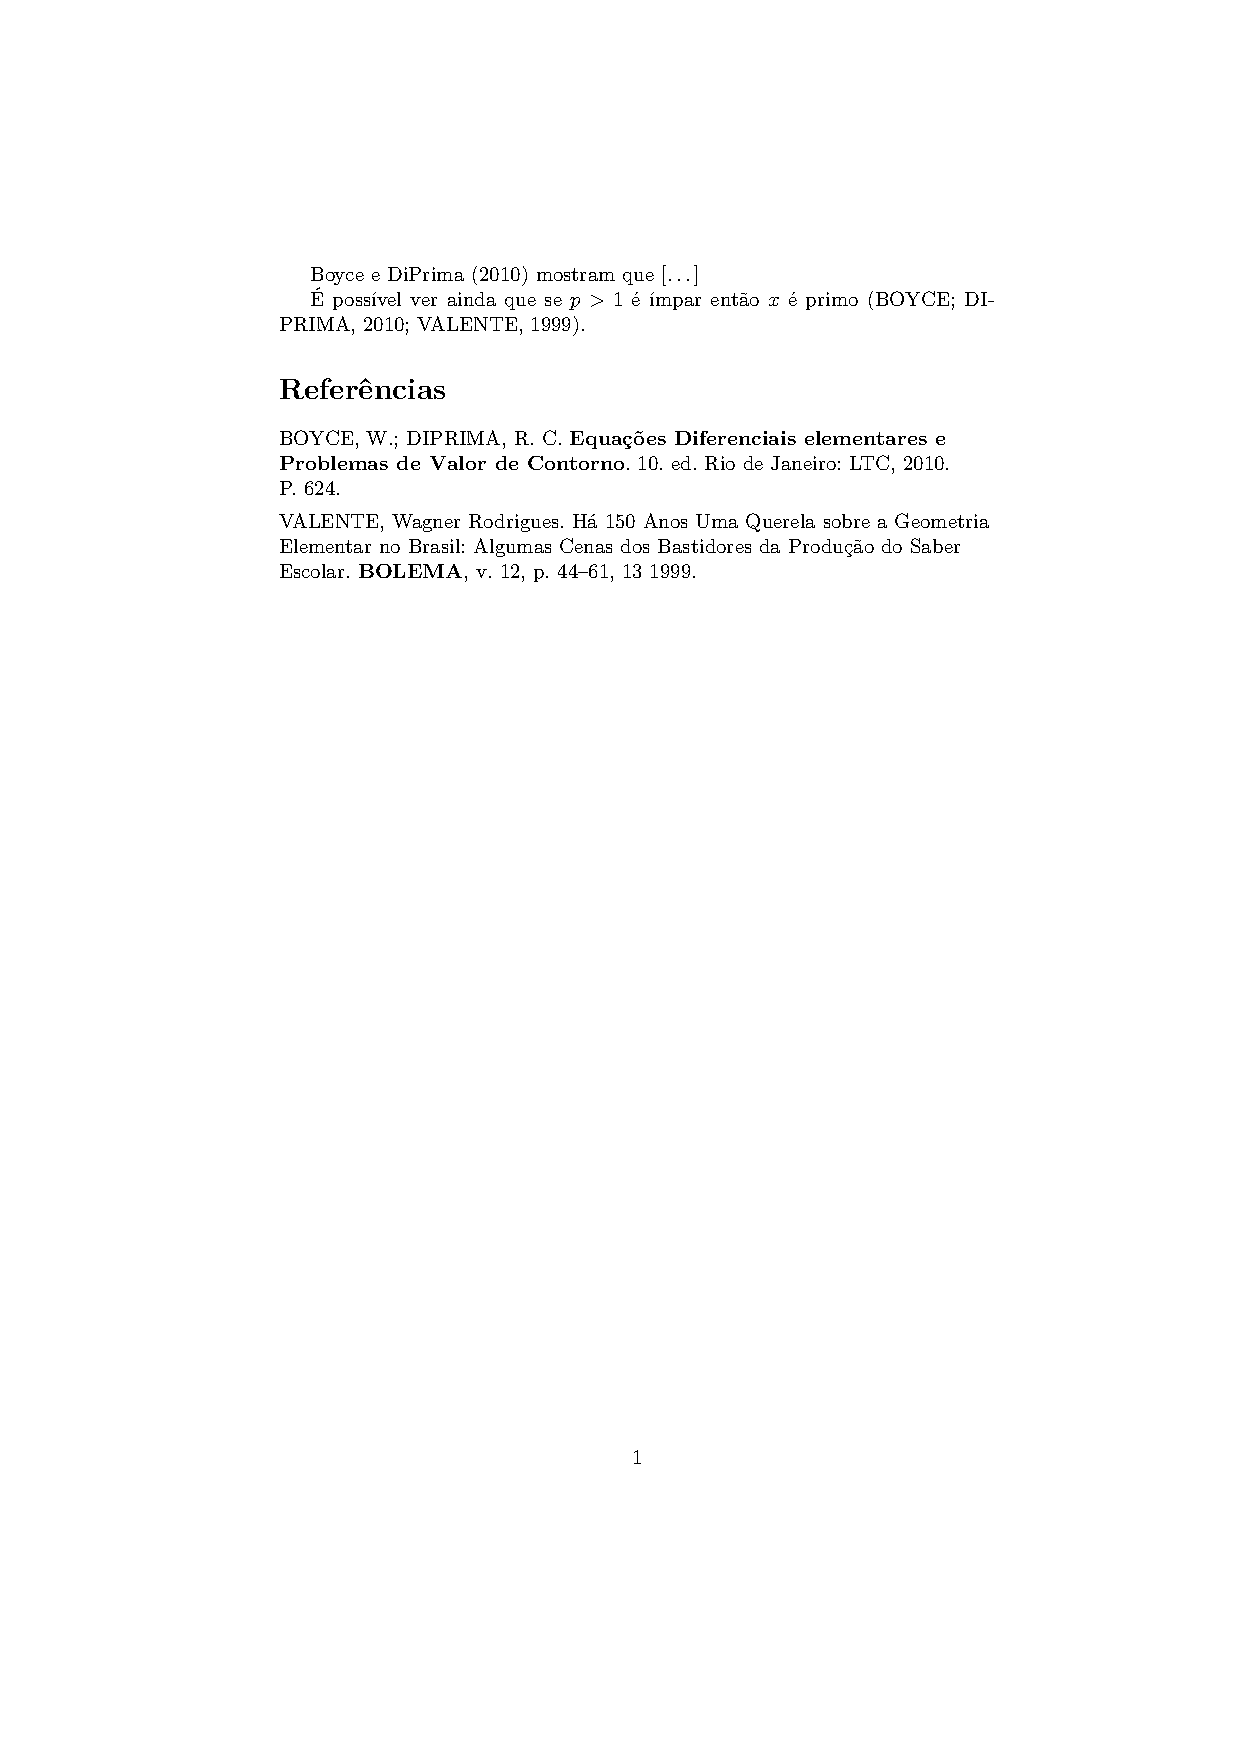
\includegraphics[width=\textwidth,clip,trim=1.8in 5in 1.5in 1in]{bib-example-abnt.pdf}
\end{minipage}
\end{frame}

%%%%%%%%%%%%%%%%%%%%%%%%%%%%%%%%%%%%%%%%%%%%%%%%%%%%%%%%%%%%%%%%%%%%%%%%%%%%%%%
%%%%%%%%%%%%%%%%%%%%%%%%%%%%%%%%%%%%%%%%%%%%%%%%%%%%%%%%%%%%%%%%%%%%%%%%%%%%%%%
%%%%%%%%%%%%%%%%%%%%%%%%%%%%%%%%%%%%%%%%%%%%%%%%%%%%%%%%%%%%%%%%%%%%%%%%%%%%%%%
\subsection{Exercício}
\begin{frame}[fragile]{Exercício: Juntando tudo}
Adicione uma imagem, uma tabela  e várias bibliografias\footnote{Inclua tipos diferentes como artigo, livro, teses, etc.} ao artigo do exercício anterior.
\begin{enumerate}
  \item Baixe os arquivos abaixo no seu computador.
  \begin{center}
    \fbox{\href{\fileuri/gerbil.jpg?dl=1}{Clique para baixar a imagem}}
    \fbox{\href{\fileuri/bib-exercise.bib?dl=1}{Clique para baixar o arquivo .bib}}
  \end{center}
  \item Adicione-os ao  Overleaf (use o menu de arquivos).
\end{enumerate}
\end{frame}

%%%%%%%%%%%%%%%%%%%%%%%%%%%%%%%%%%%%%%%%%%%%%%%%%%%%%%%%%%%%%%%%%%%%%%%%%%%%%%%
%%%%%%%%%%%%%%%%%%%%%%%%%%%%%%%%%%%%%%%%%%%%%%%%%%%%%%%%%%%%%%%%%%%%%%%%%%%%%%%
%%%%%%%%%%%%%%%%%%%%%%%%%%%%%%%%%%%%%%%%%%%%%%%%%%%%%%%%%%%%%%%%%%%%%%%%%%%%%%%
\section{E agora?}

%%%%%%%%%%%%%%%%%%%%%%%%%%%%%%%%%%%%%%%%%%%%%%%%%%%%%%%%%%%%%%%%%%%%%%%%%%%%%%%
%%%%%%%%%%%%%%%%%%%%%%%%%%%%%%%%%%%%%%%%%%%%%%%%%%%%%%%%%%%%%%%%%%%%%%%%%%%%%%%
%%%%%%%%%%%%%%%%%%%%%%%%%%%%%%%%%%%%%%%%%%%%%%%%%%%%%%%%%%%%%%%%%%%%%%%%%%%%%%%
\begin{frame}{Resumo}
\begin{multicols}{2}
\tableofcontents[currentsection]
\end{multicols}
\end{frame}

%%%%%%%%%%%%%%%%%%%%%%%%%%%%%%%%%%%%%%%%%%%%%%%%%%%%%%%%%%%%%%%%%%%%%%%%%%%%%%%
%%%%%%%%%%%%%%%%%%%%%%%%%%%%%%%%%%%%%%%%%%%%%%%%%%%%%%%%%%%%%%%%%%%%%%%%%%%%%%%
%%%%%%%%%%%%%%%%%%%%%%%%%%%%%%%%%%%%%%%%%%%%%%%%%%%%%%%%%%%%%%%%%%%%%%%%%%%%%%%
\subsection{Mais coisas legais}
\begin{frame}[fragile]{\insertsubsection}
\begin{itemize}
  \item Adicione o comando \cmdbs{tableofcontents} para gerar o sumário automaticamente a partir dos comandos  \cmdbs{section}.
  \item Mude a classe de documentos em \cmdbs{documentclass} para
  \mint{latex}!\documentclass{scrartcl} %Koma-Script!
  ou
  \mint{latex}!\documentclass[12pt]{IEEEtran} %IEEE Transactions!
  \item Defina o seu próprio comando de uma equação complicada:
\begin{exampletwouptiny}
\newcommand{\rperf}
  {\rho_{\text{perf}}}

\begin{equation}
  \rperf =
  {\bf c}'{\bf X} + \varepsilon
\end{equation}
\end{exampletwouptiny}
\end{itemize}
\end{frame}

%%%%%%%%%%%%%%%%%%%%%%%%%%%%%%%%%%%%%%%%%%%%%%%%%%%%%%%%%%%%%%%%%%%%%%%%%%%%%%%
%%%%%%%%%%%%%%%%%%%%%%%%%%%%%%%%%%%%%%%%%%%%%%%%%%%%%%%%%%%%%%%%%%%%%%%%%%%%%%%
%%%%%%%%%%%%%%%%%%%%%%%%%%%%%%%%%%%%%%%%%%%%%%%%%%%%%%%%%%%%%%%%%%%%%%%%%%%%%%%
\subsection{Mais pacotes legais}
\begin{frame}{\insertsubsection}
\begin{itemize}
  \item \bftt{beamer}: para apresentações (como esta aqui!)
  \item \bftt{todonotes}: comentários e gerenciamento listas TODO
  \item \bftt{tikz}: faça figuras sensacionais
  \item \bftt{pgfplots}: crie  gráficos em \LaTeX
  \item \bftt{listings}: imprima seu código fonte em \LaTeX
  \item \bftt{spreadtab}: crie planilhas em  \LaTeX
  \item \bftt{gchords}, \bftt{guitar}: acordes para violão e tablaturas
  \item \bftt{cwpuzzle}: para palavras cruzadas
\end{itemize}
Veja \href{https://www.overleaf.com/latex/examples}{Overleaf} ou \href{http://texample.net}{texample} para exemplos da maioria desses pacotes.
\end{frame}

%%%%%%%%%%%%%%%%%%%%%%%%%%%%%%%%%%%%%%%%%%%%%%%%%%%%%%%%%%%%%%%%%%%%%%%%%%%%%%%
%%%%%%%%%%%%%%%%%%%%%%%%%%%%%%%%%%%%%%%%%%%%%%%%%%%%%%%%%%%%%%%%%%%%%%%%%%%%%%%
%%%%%%%%%%%%%%%%%%%%%%%%%%%%%%%%%%%%%%%%%%%%%%%%%%%%%%%%%%%%%%%%%%%%%%%%%%%%%%%
\subsection{Instalando \LaTeX{}}
\begin{frame}{\insertsubsection}
\begin{itemize}
  \item Para compilar o \LaTeX{} no seu próprio computador, você vai precisar de uma \emph{distribuição} do \LaTeX{}.
  Uma distribuição inclui um programa \bftt{latex} e (tipicamente) alguns milhares de pacotes.
  \begin{itemize}
    \item No Windows: \href{http://miktex.org/}{Mik\TeX} ou \href{http://tug.org/texlive/}{\TeX Live}
    \item No Linux: \href{http://tug.org/texlive/}{\TeX Live}
    \item No Mac: \href{http://tug.org/mactex/}{Mac\TeX}
  \end{itemize}
  \item Você também vai querer utilizar um editor para \LaTeX{}. Veja \href{http://en.wikipedia.org/wiki/Comparison_of_TeX_editors}{Wikipedia} para uma lista de opções.
  \item Você também vai precisar saber mais sobre como \bftt{latex} e suas ferramentas relacionadas funcionam --- veja fontes de recursos no próximo \emph{slide}.
\end{itemize}
\end{frame}

%%%%%%%%%%%%%%%%%%%%%%%%%%%%%%%%%%%%%%%%%%%%%%%%%%%%%%%%%%%%%%%%%%%%%%%%%%%%%%%
%%%%%%%%%%%%%%%%%%%%%%%%%%%%%%%%%%%%%%%%%%%%%%%%%%%%%%%%%%%%%%%%%%%%%%%%%%%%%%%
%%%%%%%%%%%%%%%%%%%%%%%%%%%%%%%%%%%%%%%%%%%%%%%%%%%%%%%%%%%%%%%%%%%%%%%%%%%%%%%
\subsection{Recursos}
\begin{frame}{\insertsubsection}
\begin{itemize}
  \item \href{http://en.wikibooks.org/wiki/LaTeX}{The \LaTeX{} Wikibook} --- tutoriais excelentes e material de referência.
  \item \href{http://tex.stackexchange.com/}{\TeX{} Stack Exchange} --- pergunte questões e tenha respostas excelentes e rápidas.
  \item \href{http://www.latex-community.org/}{\LaTeX{} Community} --- um imenso fórum \emph{online}
  \item \href{http://ctan.org/}{Comprehensive \TeX{} Archive Network (CTAN)} --- mais de quatro mil pacotes e sua documentação
  \item \href{http://latexbr.blogspot.com.br/}{\LaTeX{} BR --- blog com dicas em português}
  \item Google em geral vai levá-lo para um dos \emph{links} acima.
\end{itemize}
\end{frame}

%%%%%%%%%%%%%%%%%%%%%%%%%%%%%%%%%%%%%%%%%%%%%%%%%%%%%%%%%%%%%%%%%%%%%%%%%%%%%%%
%%%%%%%%%%%%%%%%%%%%%%%%%%%%%%%%%%%%%%%%%%%%%%%%%%%%%%%%%%%%%%%%%%%%%%%%%%%%%%%
%%%%%%%%%%%%%%%%%%%%%%%%%%%%%%%%%%%%%%%%%%%%%%%%%%%%%%%%%%%%%%%%%%%%%%%%%%%%%%%
\begin{frame}
\begin{center}
Obrigado, e capriche nos seus próximos  \TeX{}tos!
\end{center}
\end{frame}

\end{document}

% % -- latex understands words, sentences and paragraphs

% Words are separated by one or more spaces.  Paragraphs are separated by
% one or more blank lines.  The output is not affected by adding extra
% spaces or extra blank lines to the input file.

% Double quotes are typed like this: ``quoted text''.
% Single quotes are typed like this: `single-quoted text'.

% Emphasized text is typed like this: \emph{this is emphasized}.
% Bold       text is typed like this: \textbf{this is bold}.

% -- Adding structure to your document

% \section{Hello}

% \subsection{World}

% \subsection{Foo}

% \subsubsection*{Stuff} % star form

% \subsubsection*{Results}

% -- Labels and cross-references

% \label{sec:intro}
% \label{sec:method}
% \ref{sec:method}

% --> maybe introduce the prettyref package here.

% -- Mathematics

% Inline mathematics: $x + y < 7$.

% 'Displayed' mathematics:
% \begin{equation}
% \end{equation}

% \begin{equation*}
% \end{equation*}

% \begin{align}
% \end{align}

% -- Figures

% - Need the graphicx package.

% - here we can start introducing options

% \includegraphics[width=\textwidth]{}

% - where do you find out about these options? --> link to the Wikibook

% -- Floating Figures

% \begin{figure}
% \includegraphics{...}
% \caption{\label{}Here is a caption.}
% \end{figure}

% -- Tables

% - not the nicest part of LaTeX

% \usepackage{tabularx}

% \begin{tabular}{llr}
% Item & Quantity & Price (\$) & Amount
% Widget & 1 &
% \end{tabular}

% Bonus points: check out the fp package and the spreadtab package.

% -- Document Classes

% a .cls file

% article

% some journal templates come with one

% -- Bibliographies



% -- For Typesetting Geeks

% - dashes: -, --, ---

% - ellipsis.

% - controlling spaces: ~, \ , \,, \@

% - spacing after periods (et al., etc.)

% - Nested quotation marks: ``\,`
% \vskip 2ex
% \item Use the \emph{star form} to display an equation without a number.
% \begin{exampletwouptiny}
% \begin{equation*}
% F(x) = \int_{a}^{x}{f(t) dt}
% \end{equation*}
% \end{exampletwouptiny}

% \begin{itemize}
% \item \bftt{equation} and \bftt{equation*} are called \emph{environments}.
% \begin{itemize}
%   \item The \cmdbs{begin} and \cmdbs{end} commands define the environment.
%   \item The \cmd{\$} also starts and ends an environment.
%   \item Some commands are defined only within certain environments.
%   \item Some commands behave differently in different environments.
% \end{itemize}
% \end{itemize}
% \end{block}
% \begin{center}
% \fbox{\href{http://ctan.org/}{The Comprehensive \TeX Archive Network (CTAN)}}
% \end{center}

% %%%%%%%%%%%%%%%%%%%%%%%%%%%%%%%%%%%%%%%%%%%%%%%%%%%%%%%%%%%%%%%%%%%%%%%%%%%%%%%
% %%%%%%%%%%%%%%%%%%%%%%%%%%%%%%%%%%%%%%%%%%%%%%%%%%%%%%%%%%%%%%%%%%%%%%%%%%%%%%%
% %%%%%%%%%%%%%%%%%%%%%%%%%%%%%%%%%%%%%%%%%%%%%%%%%%%%%%%%%%%%%%%%%%%%%%%%%%%%%%%
% \subsection{Typography tweaks}
% \begin{frame}{\insertsubsection}
% \begin{tabular}{lll}
% & character name & used mainly for \ldots \\\hline
% \bftt{\bs} & backslash                 & commands, tables \\
% \bftt{\{}  & open brace                & commands \\
% \bftt{\}}  & close brace               & commands \\
% \bftt{\%}  & percent sign              & comments \\
% \bftt{\#}  & hash (pound / sharp) sign & custom commands \\
% \bftt{\$}  & dollar sign               & equations \\
% \bftt{\_}  & underscore                & equations (subscripts) \\
% \bftt{\^}  & caret                     & equations (superscripts) \\
% \bftt{\&}  & ampersand                 & tables \\
% \bftt{\~}  & tilde                     & spacing \\
% \end{tabular}
% \end{frame}

% %\item We've used several environments:
% %\vskip 1ex
% %{\scriptsize
% %\begin{tabular}{ll}
% %\cmdbs{begin}\bftt{\{document\}}\ldots\cmdbs{end}\bftt{\{document\}} &
% %  document environment \\
% %\cmdbs{begin}\bftt{\{itemize\}}\ldots\cmdbs{end}\bftt{\{itemize\}} &
% %  itemized list environment \\
% %\bftt{\$\ldots\$}     & \emph{in-text} math environment \\
% %\bftt{\$\$\ldots\$\$} & \emph{displayed} math environment \\
% %\cmdbs{begin}\bftt{\{equation\}}\ldots\cmdbs{end}\bftt{\{equation\}} &
% %  displayed math environment w/ number
% %\end{tabular}
% %}

